% \documentclass[12pt, twoside]{article}
\usepackage[letterpaper, margin=1in, headsep=0.2in]{geometry}
\setlength{\headheight}{0.6in}
%\usepackage[english]{babel}
\usepackage[utf8]{inputenc}
\usepackage{microtype}
\usepackage{amsmath}
\usepackage{amssymb}
%\usepackage{amsfonts}
\usepackage[nomessages]{fp} %\FPeval{\var-name}{2*sin(pi/6)}
\usepackage{siunitx} %units in math. eg 20\milli\meter
\usepackage{yhmath} % for arcs, overparenth command
\usepackage{tikz} %graphics
\usetikzlibrary{quotes, angles, arrows, arrows.meta}
\usepackage{graphicx} %consider setting \graphicspath{{images/}}
\usepackage{parskip} %no paragraph indent
\usepackage{enumitem}
\usepackage{multicol}
\usepackage{venndiagram}

\usepackage{fancyhdr}
\pagestyle{fancy}
\fancyhf{}
\renewcommand{\headrulewidth}{0pt} % disable the underline of the header
\raggedbottom
\hfuzz=2mm %suppresses overfull box warnings

\usepackage{hyperref}

\fancyhead[LE]{\thepage}
\fancyhead[RO]{\thepage \\ Name: \hspace{4cm} \,\\}
\fancyhead[LO]{BECA / Dr. Huson / Geometry\\*  Unit 1: Segments, length, and area\\* 20 Sept 2022}

\begin{document}

\subsubsection*{1.9 Extension: Significant figures}
\emph{Significant figures are the digits in a number that are meaningful for accuracy, as opposed to zeros for place value.} See \href{https://www.mathsisfun.com/definitions/significant-digits.html}{MathIsFun definitions Significant Digits}
\begin{enumerate}
  \item Write down the number of significant digits in each value.
  \begin{multicols}{3}
    \begin{enumerate}[itemsep=1cm]
      \item 8
      \item 27
      \item 60
      \item 120
      \item 105.5
      \item 1.7320
    \end{enumerate}
  \end{multicols} \vspace{1cm}

\item Round each value to three sig figs
  \begin{multicols}{2}
    \begin{enumerate}[itemsep=0.5cm]
      \item 1,472,654 \par (population of the Bronx)
      \item $\pi$
      \item 8,804,190 \par (population of NYC)
      \item $\sqrt{2}$
    \end{enumerate}
  \end{multicols} \vspace{1cm}

\item Do the calculation two ways: round each value to three sig figs before calculating versus round only at the end.
  \begin{multicols}{2}
    \begin{enumerate}[itemsep=3cm]
      \item $39.37^2-1510$
      \item $1.2548^2 \pi$
      \item $39.37^2-1510$
      \item $1.2548^2 \pi$
    \end{enumerate}
  \end{multicols} \vspace{1cm}
  What do you notice. In calculations, when should values be rounded?

\newpage
\item A large rectangle is divided by a vertical line into a square and a smaller rectangle, as shown. Its height is 7 and base $x+3$, as marked.
\begin{multicols}{2}
  \begin{tikzpicture}
    \draw[thick] (0,0) rectangle (6,4);
    \draw[thick] (4,0) -- (4,4);
    \node at (6.4,2.2){7};
    \node at (2,-0.4){$x$};
    \node at (5,-0.4){3};
  \end{tikzpicture}
  \begin{enumerate}
    \item Find the area of the square. \vspace{2cm}
    \item Find the perimeter of large rectangle.
    \end{enumerate}
  \end{multicols} \vspace{1cm}

\item Find the \emph{area} of the shape shown below composed of a rectangle and two semi-circular caps. Round the result to three sig figs.
\begin{flushright}
\begin{tikzpicture}[scale=.635]
  \draw[help lines] (-1,-1) grid (7,7);
  \draw[thick, ->] (-1.2,0) -- (7.4,0) node [below right] {$x$};
  \draw[thick, ->] (0,-1.2)--(0,7.4) node [left] {$y$};
  \draw[thick] (2,2)--(5,2)--(5,4)--(2,4)--cycle;
  \draw[thick] (2,4) arc (90:270:1);
  \draw[thick] (5,2) arc (-90:90:1);
\end{tikzpicture}
\end{flushright} \vspace{2cm}

\item Given that the distance from the earth to the sun is 94.297 million miles. Find the circumference of the earth's orbit around the sun. (leave your result in scientific notation rounded to three sig figs)


\end{enumerate}
\end{document}